% AUTHOR: Sina Atalay
% LICENSE: https://github.com/sinaatalay/rendercv/blob/main/LICENSE

\documentclass[10pt, letterpaper]{article}

% Packages:
\usepackage[
        ignoreheadfoot, % set margins without considering header and footer
        top=2 cm, % seperation between body and page edge from the top
        bottom=2 cm, % seperation between body and page edge from the bottom
        left=2 cm, % seperation between body and page edge from the left
        right=2 cm, % seperation between body and page edge from the right
        footskip=1.0 cm, % seperation between body and footer
        % showframe % for debugging 
    ]{geometry} % for adjusting page geometry
\usepackage[explicit]{titlesec} % for customizing section titles
\usepackage{tabularx} % for making tables with fixed width columns
\usepackage{array} % tabularx requires this
\usepackage[dvipsnames]{xcolor} % for coloring text
\definecolor{primaryColor}{RGB}{0, 79, 144} % define primary color
\usepackage{enumitem} % for customizing lists
\usepackage{fontawesome5} % for using icons
\usepackage{amsmath} % for math
\usepackage{graphicx}
\usepackage[
    pdftitle={Alessandro Mileto's CV},
    pdfauthor={Alessandro Mileto},
    colorlinks=true,
    urlcolor=primaryColor
]{hyperref} % for links, metadata and bookmarks
\usepackage[pscoord]{eso-pic} % for floating text on the page
\usepackage{calc} % for calculating lengths
\usepackage{bookmark} % for bookmarks
\usepackage{lastpage} % for getting the total number of pages
\usepackage[default, type1]{sourcesanspro} % for using source sans 3 font
\usepackage{ifthen}

% Some settings:
\pagestyle{empty} % no header or footer
\setcounter{secnumdepth}{0} % no section numbering
\setlength{\parindent}{0pt} % no indentation
\setlength{\topskip}{0pt} % no top skip
\makeatletter
\let\ps@customFooterStyle\ps@plain% Copy the plain style to customFooterStyle
\usepackage{etoolbox}
\patchcmd{\ps@customFooterStyle}{\thepage}{
    \color{gray}\textit{\small Alessandro Mileto - Page \thepage{} of \pageref*{LastPage}}
}{}{} % replace number by desired string

\makeatother
\pagestyle{customFooterStyle}

\titleformat{\section}{
        % make the font size of the section title large and color it with the primary color
        \Large\color{primaryColor}
    }{
    }{
    }{
        % print bold title, give 0.15 cm space and draw a line of 0.8 pt thickness
        % from the end of the title to the end of the body
        \textbf{#1}\hspace{0.15cm}\titlerule[0.8pt]\hspace{-0.1cm}
    }[] % section title formatting

\titlespacing{\section}{
        % left space:
        0pt
    }{
        % top space:
        0.3 cm
    }{
        % bottom space:
        0.2 cm
    } % section title spacing

\newcolumntype{L}[1]{
    >{\raggedright\let\newline\\\arraybackslash\hspace{0pt}}p{#1}
} % left-aligned fixed width column type
\newcolumntype{R}[1]{
    >{\raggedleft\let\newline\\\arraybackslash\hspace{0pt}}p{#1}
} % right-aligned fixed width column type
\newcolumntype{K}[1]{
    >{\let\newline\\\arraybackslash\hspace{0pt}}X
} % justified flexible width column type
\setlength\tabcolsep{-1.5pt} % no space between columns
\newenvironment{highlights}{
        \begin{itemize}[
                topsep=0pt,
                parsep=0.10 cm,
                partopsep=0pt,
                itemsep=0pt,
                after=\vspace{-1\baselineskip},
                leftmargin=0.4 cm + 3pt
            ]
    }{
        \end{itemize}
    } % new environment for highlights

\newenvironment{header}{
        \setlength{\topsep}{0pt}\par\kern\topsep\centering\color{primaryColor}\linespread{1.5}
    }{
        \par\kern\topsep
    } % new environment for the header

\newcommand{\placelastupdatedtext}{% \placetextbox{<horizontal pos>}{<vertical pos>}{<stuff>}
  \AddToShipoutPictureFG*{% Add <stuff> to current page foreground
    \put(
        \LenToUnit{\paperwidth-2 cm-0.2 cm+0.05cm},
        \LenToUnit{\paperheight-1.0 cm}
    ){\vtop{{\null}\makebox[0pt][c]{
        \small\color{gray}\textit{Last updated in April 2024}\hspace{\widthof{Last updated in April 2024}}
    }}}%
  }%
}%

% save the original href command in a new command:
\let\hrefWithoutArrow\href
 % new command for external links:
\renewcommand{\href}[2]{\hrefWithoutArrow{#1}{\mbox{\ifthenelse{\equal{#2}{}}{ }{#2 }\raisebox{.15ex}{\footnotesize \faExternalLink*}}}}

\let\originalTabularx\tabularx
\let\originalEndTabularx\endtabularx

\renewenvironment{tabularx}{\bgroup\centering\originalTabularx}{\originalEndTabularx\par\egroup}

% For TextEntrys (see https://tex.stackexchange.com/a/600/287984):
\def\changemargin#1#2{\list{}{\rightmargin#2\leftmargin#1\topsep=0pt\itemsep=0pt\parsep=0pt\parskip=0pt\labelwidth=0pt\itemindent=0pt\labelsep=0pt}\item[]}
\let\endchangemargin=\endlist 

% Ensure that generate pdf is machine readable/ATS parsable
\pdfgentounicode=1

\begin{document}

    
    \begin{header}
        \fontsize{30 pt}{30 pt}
        \textbf{Alessandro Mileto}

        \vspace{0.3 cm}
\begin{figure}[h]
    \centering
    \begin{minipage}{0.2\textwidth}
        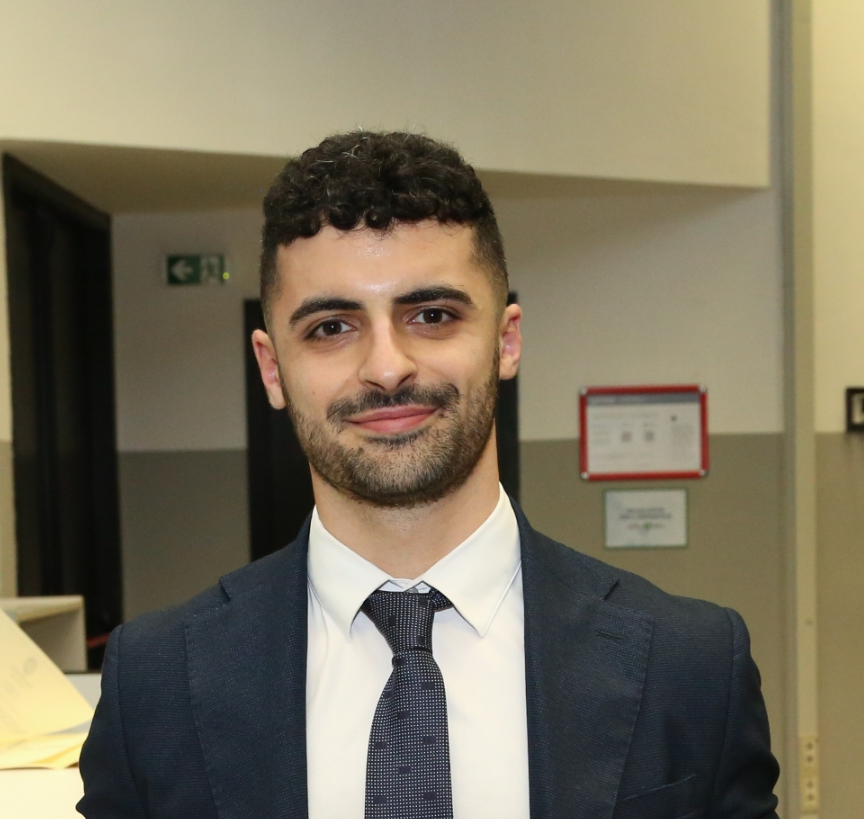
\includegraphics[width=\textwidth]{io.png}
    \end{minipage}%
    \hspace{0.3cm }
    \begin{minipage}{0.6\textwidth}
        \begin{samepage}
        \raggedright
        I am Alessandro, a Computer Engineer passionate about \textit{systems security and engineering}.  I did research on OS virtualization and hypervisor-based OS security. In the years, I also learned about Offensive Security techniques, Cryptography, Machine and Deep Learning and much more and I feel ready to apply my skills to tackle real-world challenges!
        \end{samepage}
    \end{minipage}
\end{figure}
        \normalsize
        \mbox{\hrefWithoutArrow{tel:+393669549870}{{\footnotesize\faPhone*}\hspace*{0.13cm}+39 366 9549870}}
        \hspace*{0.5 cm}
        \mbox{\hrefWithoutArrow{mailto:alessandromileto22@gmail.com}{{\small\faEnvelope[regular]}\hspace*{0.13cm}alessandromileto22@gmail.com}}
        \hspace*{0.5 cm}
        \mbox{{\small\faMapMarker*}\hspace*{0.13cm}Milan, Italy}
        \hspace*{0.5 cm}
        % \mbox{\hrefWithoutArrow{https://yourwebsite.com/}{{\small\faLink}\hspace*{0.13cm}yourwebsite.com}}
        % \hspace*{0.5 cm}
        \mbox{\hrefWithoutArrow{https://linkedin.com/in/alessandro-mileto}{{\small\faLinkedinIn}\hspace*{0.13cm}alessandro-mileto}}
        \hspace*{0.5 cm}
        \mbox{\hrefWithoutArrow{https://github.com/ubersandro}{{\small\faGithub}\hspace*{0.13cm}ubersandro}}
        \hspace*{0.5 cm}
    \end{header}

    \vspace{0.3 cm}


    % \section{Summary}

    %     \begin{changemargin}{0.2 cm}{0.2 cm}
    %      
    %     \end{changemargin}





    
    \section{Education}

    \begin{tabularx}{
            \textwidth-0.4 cm-0.13cm
        }{
            L{0.85cm}
            K{0.2 cm}
            R{4.1 cm}
        }
            \textbf{MS}
            &
            
            \textbf{Politecnico di Milano} - Computer Science and Engineering (Ingegneria Informatica) 

            \vspace{0.10 cm}

            \begin{highlights}
                \item Grade: With Honors
                \item GPA: 28.95/30 (\href{https://linkedin.com/in/alessandro-mileto}{Transcript})
                % \item \textbf{Coursework:} Classic AI, Machine and Deep Learning, Computer Security, Offensive and Defensive Cybersecurity, Numerical Analysis and Scientific Computing, Network Science and Graph Analysis, Advanced Operating Systems, Embedded Systems, Database Systems, Formal Languages, Compilers and Theoretical Computer Science, Advanced Computer Architectures, Applied Cryptography and Architectures for Computer Security, Advanced topics in Mathematical Logics and Distributed Systems. 
                \item \textbf{Thesis title}: \textit{On the Performance of Hypervisor-based Memory Monitoring for Code Unpacking Detection}
                % \begin{itemize}
                %     \item [] The thesis investigates the cost of Hypervisor-based Monitoring leveraging Virtual Machine Introspection and hardware support. We study the performance penalty on memory accesses of hooking, and the impact of different strategies for handling the Semantic Gap to follow processes execution to detect code unpacking. In the end, we propose guidelines for efficient HV-based monitoring implementation. 
                % \end{itemize}
            \end{highlights}
            &
            

            Sept. 2021 to April 2024
            Milan, Italy
        \end{tabularx}
\vspace{0.1cm}   
  \begin{tabularx}{
            \textwidth-0.4 cm-0.13cm
        }{
            L{0.85cm}
            K{0.2 cm}
            R{4.1 cm}
        }
            \textbf{Ext}
            &
            
            \textbf{       Max Planck Society} - Cornell, Maryland, Max Planck Pre-doctoral Summer School
            
            \vspace{0.20 cm}

            \begin{highlights}
                \item \textbf{Selected} for attendance among about 100 candidates over more than 500 
                \item Pre-doctoral summer school jointly organized by \textbf{Cornell University, Maryland University, Max Planck Institute.}
                % \item Where: Max Planck Institute for Software Systems, Saarbrücken, Germany
                % \item \textbf{Classes:}  Software Verification, Quantum Computing, Parallel Graph Algorithms, Human-centric Security and Privacy, Optic Networks, ML Performativity, LLMs and automated Q\&A, Robotics for Healthcare, how to talk in public and to write research papers. 
            \end{highlights}
            &
            

                August 2023                               
                
            Saarbrücken, Germany
        \end{tabularx}
\begin{tabularx}{
            \textwidth-0.4 cm-0.13cm
        }{
            L{0.85cm}
            K{0.2 cm}
            R{4.1 cm}
        }
            \textbf{Ext}
            &
            
            \textbf{NECST Camp} - NECSTLab, Politecnico di Milano

            \vspace{0.10 cm}
\begin{highlights}
    \item Extra-curricular activities to promote personal and professional growth curated by Professor Marco Santambrogio of Politecnico di Milano.
    \item Soft skills: social intelligence, psychology and pitching
    \item Hard skills: hardware accelerators design (Vivado for LLS, Vitis for HLS, Vitis AI)
\end{highlights}
            
            &
            

            Sept. 2022 to January 2023
            Milan, Italy
        \end{tabularx}
% \vspace{0.1cm}
        \vspace{0.1cm}
        \begin{tabularx}{
            \textwidth-0.4 cm-0.13cm
        }{
            L{0.85cm}
            K{0.2 cm}
            R{4.1 cm}
        }
            \textbf{BS}
            &
            \textbf{Università della Calabria} - Computer Science and Engineering (Ingegneria Informatica) 

            \vspace{0.20 cm}

            \begin{highlights}
            \item Grade: With Honors (and Academic Mention) 
                \item GPA: 29.02/30 (\href{https://linkedin.com/in/alessandro-mileto}{Transcript})
                % \item \textbf{Coursework:} Software Engineering and Object-Oriented Programming, Automation and Control Theory, Computer Networks, Mathematical Analysis, Probability and Statistics with a strong focus on Queue Theory, Operating Systems and Computer Architectures
                \item \textbf{Thesis title}: \textit{Studio della Sicurezza delle Reti 5G (On the Security of 5G Networks). } 
                % \begin{itemize}
                %     \item [] The thesis surveys 5G networks security ranging from RAN Systems to Software Defined Networking and Network Function Virtualization. It delves into the pitfalls and criticalities identified in the literature in the context of several novel 5G use cases and reports mitigations. 
                % \end{itemize}
            \end{highlights}
            &
            

            Sept. 2018 to Sept. 2021
            Cosenza, Italy
        \end{tabularx}
    
    \section{Working Experience}

%         \begingroup\leftskip=0.2 cm
%         \advance\csname @rightskip\endcsname 0.2 cm
%         \advance\rightskip 0.2 cm
% \begin{highlights}
    

%     \item    
    
% \end{highlights}
        
\begin{tabularx}{
    \textwidth-0.4 cm-0.13cm
}{
    L{2cm}
    K{0.85 cm}
    R{4.1 cm}
}
    \textbf{Intership}
    &
    \textbf{University of California Santa Barbara} - Research Associate 

    \vspace{0.20 cm}

    \begin{highlights}
    \item[] I will join SECLAB to work as a cybersecurity researcher (field to be defined).
    \end{highlights}
    &

    Nov. 2024 to April 2025

    Santa Barbara, 

    California, USA
\end{tabularx}     

\begin{tabularx}{
    \textwidth-0.4 cm-0.13cm
}{
    L{2cm}
    K{0.85 cm}
    R{4.1 cm}
}
    \textbf{Collab}
    &
    \textbf{Fiscal Focus} - Consultant

    \vspace{0.20 cm}

    \begin{highlights}
    \item[] I realized two digital Courses about\textbf{ Cloud Computing and Network Security} within the “Industria 4.0” project financed by European Union and promoted by Italian Government.
    \end{highlights}
    &

    Feb. 2021 - May 2021

    via Alemanni 1,
    
    Pianopoli(CZ), 
    
    88040
\end{tabularx}     


    \section{Hackathons and CTFs}

        \begin{tabularx}{
            \textwidth-0.4 cm-0.13cm
        }{
            K{0.2 cm}
            R{4.1 cm}
        }
            \textbf{Start Hack 2024}, Start Global Hackathon

            \vspace{0.10 cm}

            \begin{highlights}
                \item Hackathon about innovation in sustainable agriculture, finance education, tourism, and climate change management. 
                \item We worked on a study case by Syngenta. We proposed Spring Sprout, an app to gamify learning about agriculture with tailor-made insights for learning, challenges, quizzes, recommendations on how to grow crops and contrast diseases
                \item \href{https://github.com/AlessandroCogollo/StartHack2024/}{Link}: https://github.com/AlessandroCogollo/StartHack2024/
            \end{highlights}
            &
            St. Gallen, Switzerland

            March 2024

            36 hours
        \end{tabularx}

        \vspace{0.2 cm}
 \begin{tabularx}{
            \textwidth-0.4 cm-0.13cm
        }{
            K{0.2 cm}
            R{4.1 cm}
        }
            \textbf{GDSC AI Hackathon}, Google Developers Students Club's hackathon

            \vspace{0.10 cm}

            \begin{highlights}
                \item Hackathon about the use of AI to support education
                \item Proposed LearningDuck, an app to suggest students how to approach learning about new topics, starting from AI-generated mindmaps, quizzes, solutions, assessments, and remarks on progress done.  
                \item \href{https://github.com/NicholasNicolis/GDSC-AI-SpicyLionArancini}{Link:} https://github.com/NicholasNicolis/GDSC-AI-SpicyLionArancini
            \end{highlights}
            &
            Milan, Italy

            April 2024

            24 hours
        \end{tabularx}
       

\begin{tabularx}{
            \textwidth-0.4 cm-0.13cm
        }{
            K{0.2 cm}
            R{4.1 cm}
        }
            \textbf{0ctf}, DEF CON pre-qualifier CTF (Capture The Flag) 

            \vspace{0.10 cm}

            \begin{highlights}
                \item Played with "Mhackeroni", the biggest Italian hacking super-group under the nickname "ubersandro".
                \item Worked on Mac OS faulty driver exploitation
               \item \href{https://ctftime.org/event/2073/}{Link}: https://ctftime.org/event/2073/
            \end{highlights}
            &
            Milan, Italy

            December 2023

            48 hours
        \end{tabularx}
\begin{tabularx}{
            \textwidth-0.4 cm-0.13cm
        }{
            K{0.2 cm}
            R{4.1 cm}
        }
            \textbf{Nautilus DEF CON Quals '24}, DEF CON qualifier CTF (Capture The Flag) 

            \vspace{0.10 cm}

            \begin{highlights}
                \item Played with "Mhackeroni", the biggest Italian hacking super-group under the nickname "ubersandro" and \textbf{qualified} for the finals. 
                \item Worked on binary exploitation, reverse engineering. 
               \item \href{https://nautilus.institute/}{Link}: https://nautilus.institute/
            \end{highlights}
            &
            Milan, Italy

            May 2024

            48 hours
        \end{tabularx}

    
    \section{Projects}

        \begin{tabularx}{
            \textwidth-0.4 cm-0.13cm
        }{
            K{0.2 cm}
            R{4.1 cm}
        }
            \textbf{Artificial Neural Networks challenges}

            \vspace{0.10 cm}
            Two challenges: 
            \begin{highlights}
                \item Object Recognition and Classification (CNN, quasi-SVM), Data Augmentation (SMOTE, re-sampling, etc.).
                \item Time Series Classification
                (LSTM, RNN, GRU, 1D-CNN), and Data Augmentation (re-sampling, interpolation etc.).  
            \end{highlights}
            
            &
        
            Sep. 2022
        \end{tabularx}
\href{https://github.com/ubersandro/annHomework1}{Link}: https://github.com/ubersandro/annHomework1 

\href{https://github.com/ubersandro/annHomework2}{Link}: https://github.com/ubersandro/annHomework2
        \vspace{0.2 cm}

        \begin{tabularx}{
            \textwidth-0.4 cm-0.13cm
        }{
            K{0.2 cm}
            R{4.1 cm}
        }
            \textbf{GANs on FPGA}

            \vspace{0.10 cm}

            \begin{highlights}
                \item I accelerated the generation of images on Artix 7 FPGA using Xilinx Vitis AI, Tensorflow and PYNQ.  
            \end{highlights}
            
            &
        
            Sep. 2022
        \end{tabularx}
        \href{https://github.com/ubersandro/GANs-on-FPGA}{Link}: https://github.com/ubersandro/GANs-on-FPGA

        \begin{tabularx}{
            \textwidth-0.4 cm-0.13cm
        }{
            K{0.2 cm}
            R{4.1 cm}
        }
            \textbf{Network Analysis on PGP users dataset}

            \vspace{0.10 cm}

            \begin{highlights}
                \item I worked on NetworkX and Gephi to extract insights and data from the biggest connected component of the PGP users network and analyze them. 
            \end{highlights}
            &
        
            Sep. 2022
        \end{tabularx}
        \href{https://github.com/ubersandro/PGPusers-dataset-analysis}{Link}: https://github.com/ubersandro/PGPusers-dataset-analysis

        \vspace{0.2 cm}

    


    \section{Languages} 
    \begingroup\leftskip=0.2 cm
        \advance\csname @rightskip\endcsname 0.2 cm
        \advance\rightskip 0.2 cm
\begin{highlights}
    \item \textbf{Italian} (mother tongue)
    \item \textbf{English} (C1 Advanced Certificate in English released by Cambridge Assessment in 2017).
\end{highlights}

\vspace{0.3cm}

    \section{Technologies}

        \begingroup\leftskip=0.2 cm
        \advance\csname @rightskip\endcsname 0.2 cm
        \advance\rightskip 0.2 cm

        \textbf{Languages:} C, C++ , Java, Python, SQL, Bash, MATLAB  \par\endgroup

        \vspace{0.2 cm}
        \begingroup\leftskip=0.2 cm
        \advance\csname @rightskip\endcsname 0.2 cm
        \advance\rightskip 0.2 cm

        \textbf{Software:} Visual Studio, Eclipse, MariaDB, IntelliJ, MATLAB, Linux \par\endgroup

I authorise the treatment of my personal data in accordance with Art. 13 of D. Lgs. 196/2003 and of Art. 13 GDPR 679/16. 
\end{document}